\documentclass{standalone}
\usepackage{tikz}
\usetikzlibrary{patterns, positioning}
\usepackage[sfdefault]{ClearSans} %% option 'sfdefault' activates Clear Sans as the default text font
\usepackage[T1]{fontenc}

\begin{document}
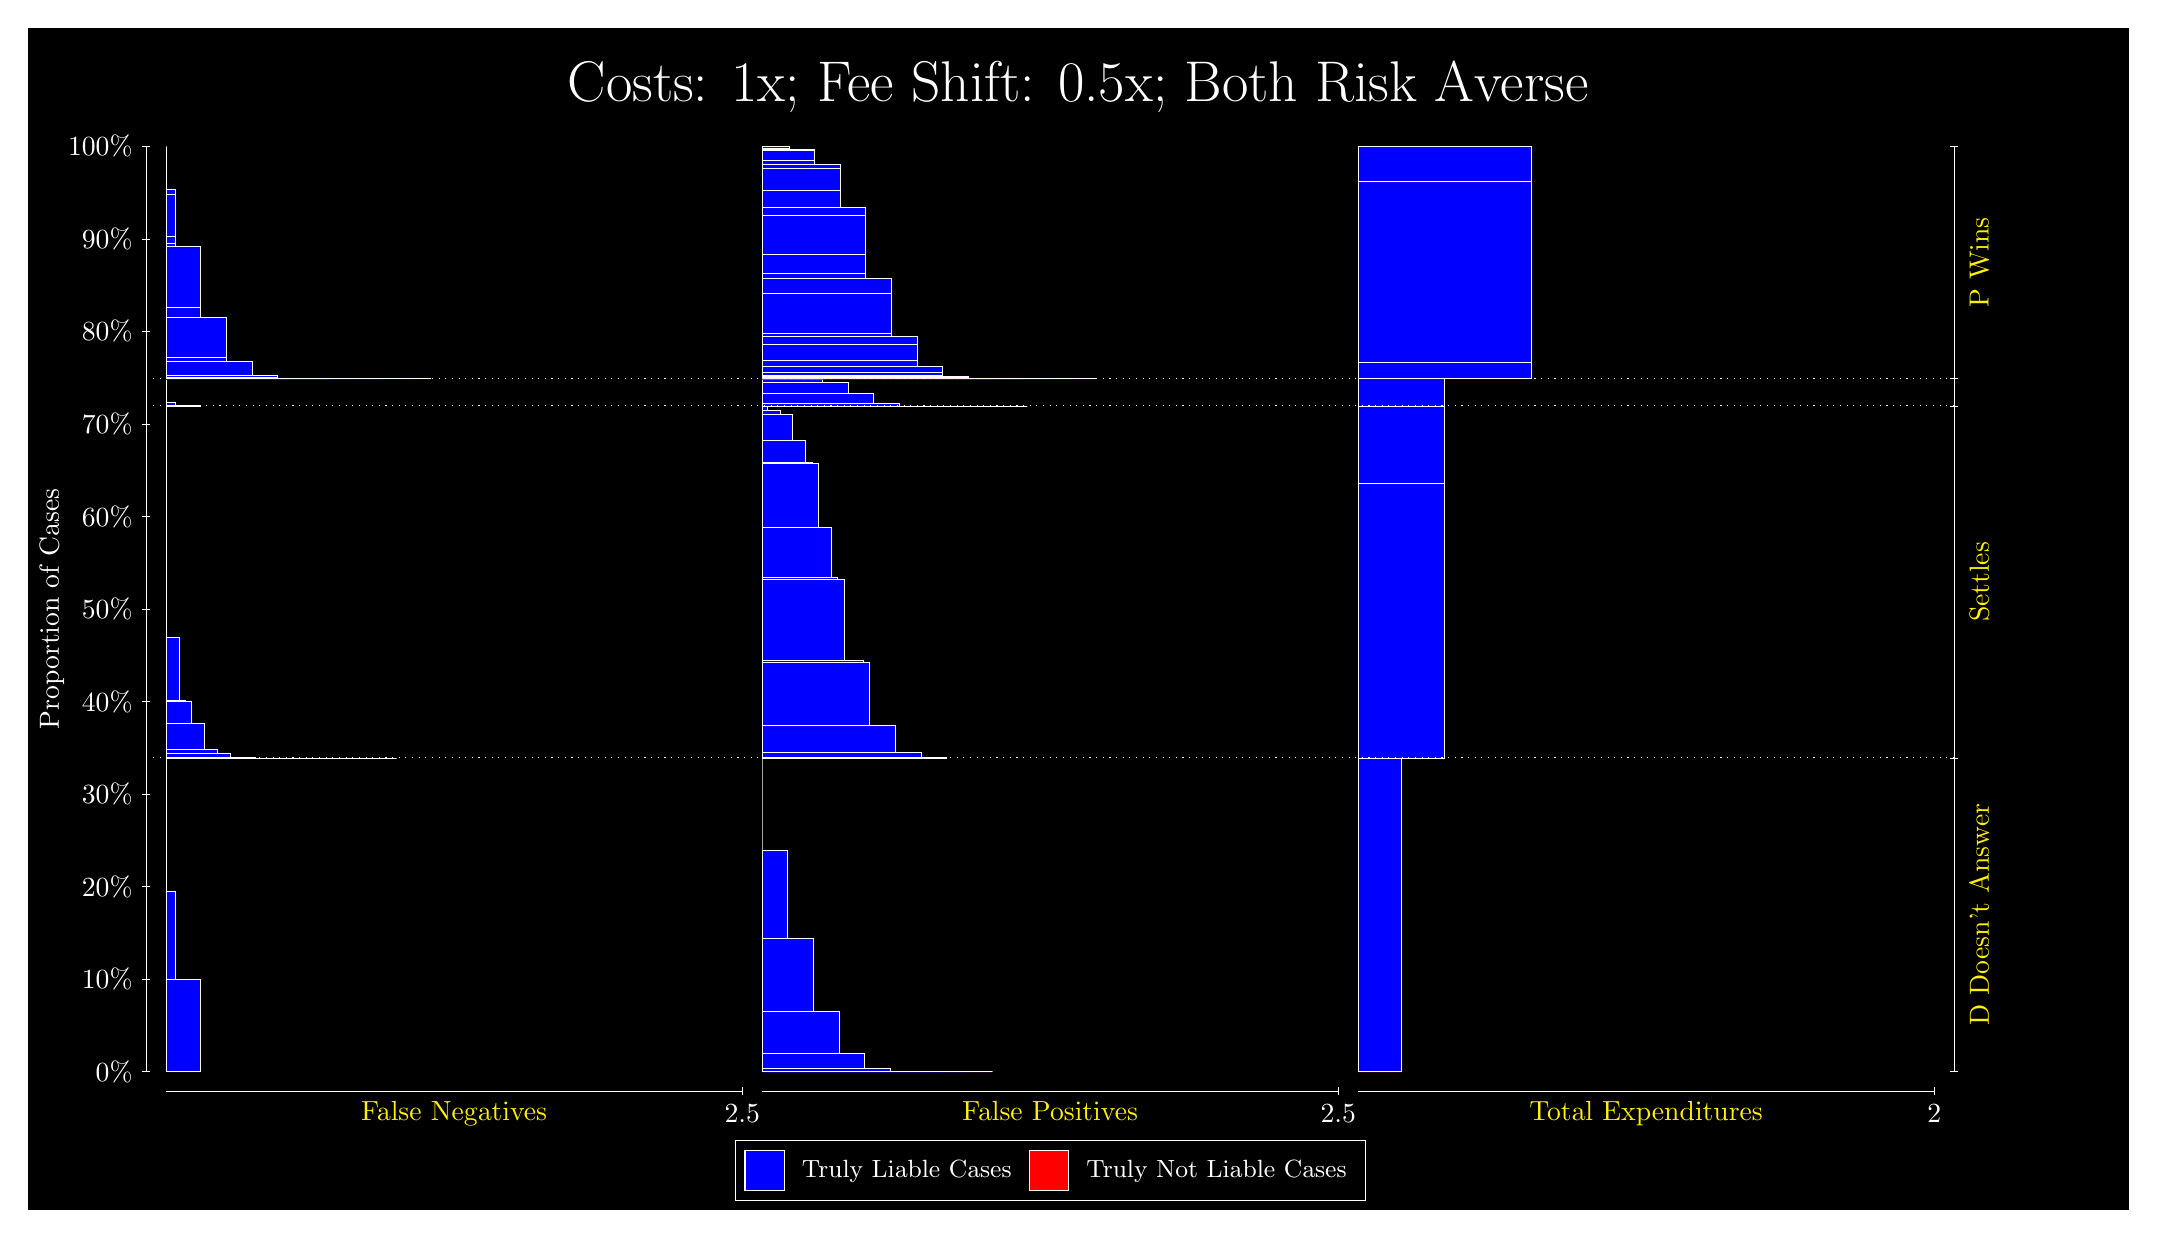
\begin{tikzpicture}
\draw[fill=black] (0,0) rectangle (26.667,15);
\draw[text=white] (0,13.5) rectangle (26.667,15) node[midway] {\huge Costs: 1x; Fee Shift: 0.5x; Both Risk Averse};
\draw[white, very thin] (1.5,1.75) -- (1.5,13.5);
\node[rotate=90, text=white, anchor=center] at (0.3, 7.625) {Proportion of Cases};
\draw[white, very thin] (1.45,1.75) -- (1.55,1.75);
\node[text=white, anchor=east] at (1.45, 1.75) {0\%};
\draw[white, very thin] (1.45,2.925) -- (1.55,2.925);
\node[text=white, anchor=east] at (1.45, 2.925) {10\%};
\draw[white, very thin] (1.45,4.1) -- (1.55,4.1);
\node[text=white, anchor=east] at (1.45, 4.1) {20\%};
\draw[white, very thin] (1.45,5.275) -- (1.55,5.275);
\node[text=white, anchor=east] at (1.45, 5.275) {30\%};
\draw[white, very thin] (1.45,6.45) -- (1.55,6.45);
\node[text=white, anchor=east] at (1.45, 6.45) {40\%};
\draw[white, very thin] (1.45,7.625) -- (1.55,7.625);
\node[text=white, anchor=east] at (1.45, 7.625) {50\%};
\draw[white, very thin] (1.45,8.8) -- (1.55,8.8);
\node[text=white, anchor=east] at (1.45, 8.8) {60\%};
\draw[white, very thin] (1.45,9.975) -- (1.55,9.975);
\node[text=white, anchor=east] at (1.45, 9.975) {70\%};
\draw[white, very thin] (1.45,11.15) -- (1.55,11.15);
\node[text=white, anchor=east] at (1.45, 11.15) {80\%};
\draw[white, very thin] (1.45,12.325) -- (1.55,12.325);
\node[text=white, anchor=east] at (1.45, 12.325) {90\%};
\draw[white, very thin] (1.45,13.5) -- (1.55,13.5);
\node[text=white, anchor=east] at (1.45, 13.5) {100\%};

\draw[white, very thin] (24.457,1.75) -- (24.457,13.5);
\draw[white, very thin] (24.407,1.75) -- (24.507,1.75);
\node[anchor=west] at (24.407, 1.75) {};
\draw[white, very thin] (24.407,5.7346) -- (24.507,5.7346);
\node[anchor=west] at (24.407, 5.7346) {};
\draw[white, very thin] (24.407,10.203) -- (24.507,10.203);
\node[anchor=west] at (24.407, 10.203) {};
\draw[white, very thin] (24.407,10.549) -- (24.507,10.549);
\node[anchor=west] at (24.407, 10.549) {};
\draw[white, very thin] (24.407,13.5) -- (24.507,13.5);
\node[anchor=west] at (24.407, 13.5) {};

\draw[white, very thin, fill=blue] (1.75,1.75) rectangle (2.1891,2.9185);
\draw[white, very thin, fill=blue] (1.75,2.9185) rectangle (1.8638,4.0397);
\draw[white, very thin, fill=red] (1.75,4.0397) rectangle (1.75,4.0397);
\draw[white, very thin, fill=blue] (1.75,4.0397) rectangle (1.75,5.7346);
\draw[white, very thin, fill=blue] (1.75,5.7346) rectangle (4.6775,5.7346);
\draw[white, very thin, fill=blue] (1.75,5.7346) rectangle (4.3523,5.7346);
\draw[white, very thin, fill=blue] (1.75,5.7346) rectangle (4.027,5.7346);
\draw[white, very thin, fill=blue] (1.75,5.7346) rectangle (3.9457,5.7346);
\draw[white, very thin, fill=blue] (1.75,5.7346) rectangle (3.7017,5.7346);
\draw[white, very thin, fill=blue] (1.75,5.7346) rectangle (3.6204,5.7346);
\draw[white, very thin, fill=blue] (1.75,5.7346) rectangle (3.3764,5.7346);
\draw[white, very thin, fill=blue] (1.75,5.7346) rectangle (3.2951,5.7346);
\draw[white, very thin, fill=blue] (1.75,5.7346) rectangle (3.2138,5.7346);
\draw[white, very thin, fill=blue] (1.75,5.7346) rectangle (3.0511,5.7346);
\draw[white, very thin, fill=blue] (1.75,5.7346) rectangle (2.9698,5.7346);
\draw[white, very thin, fill=blue] (1.75,5.7346) rectangle (2.8885,5.737);
\draw[white, very thin, fill=blue] (1.75,5.737) rectangle (2.7258,5.7391);
\draw[white, very thin, fill=blue] (1.75,5.7391) rectangle (2.6445,5.7392);
\draw[white, very thin, fill=blue] (1.75,5.7392) rectangle (2.5632,5.7907);
\draw[white, very thin, fill=blue] (1.75,5.7907) rectangle (2.4006,5.8401);
\draw[white, very thin, fill=blue] (1.75,5.8401) rectangle (2.3192,5.8403);
\draw[white, very thin, fill=blue] (1.75,5.8403) rectangle (2.2379,6.1734);
\draw[white, very thin, fill=blue] (1.75,6.1734) rectangle (2.0753,6.456);
\draw[white, very thin, fill=blue] (1.75,6.456) rectangle (1.994,6.4608);
\draw[white, very thin, fill=blue] (1.75,6.4608) rectangle (1.9126,7.2697);
\draw[white, very thin, fill=red] (1.75,7.2697) rectangle (1.75,7.2697);
\draw[white, very thin, fill=blue] (1.75,7.2697) rectangle (1.75,10.203);
\draw[white, very thin, fill=blue] (1.75,10.203) rectangle (2.1891,10.209);
\draw[white, very thin, fill=blue] (1.75,10.209) rectangle (1.8638,10.253);
\draw[white, very thin, fill=red] (1.75,10.253) rectangle (1.75,10.253);
\draw[white, very thin, fill=blue] (1.75,10.253) rectangle (1.75,10.549);
\draw[white, very thin, fill=blue] (1.75,10.549) rectangle (5.1167,10.549);
\draw[white, very thin, fill=blue] (1.75,10.549) rectangle (4.7914,10.549);
\draw[white, very thin, fill=blue] (1.75,10.549) rectangle (4.7914,10.549);
\draw[white, very thin, fill=blue] (1.75,10.549) rectangle (4.4661,10.549);
\draw[white, very thin, fill=blue] (1.75,10.549) rectangle (4.4661,10.549);
\draw[white, very thin, fill=blue] (1.75,10.549) rectangle (4.1408,10.549);
\draw[white, very thin, fill=blue] (1.75,10.549) rectangle (3.8155,10.549);
\draw[white, very thin, fill=blue] (1.75,10.549) rectangle (3.8155,10.55);
\draw[white, very thin, fill=blue] (1.75,10.55) rectangle (3.4903,10.554);
\draw[white, very thin, fill=blue] (1.75,10.554) rectangle (3.165,10.562);
\draw[white, very thin, fill=blue] (1.75,10.562) rectangle (3.165,10.587);
\draw[white, very thin, fill=blue] (1.75,10.587) rectangle (2.8397,10.772);
\draw[white, very thin, fill=blue] (1.75,10.772) rectangle (2.5144,10.817);
\draw[white, very thin, fill=blue] (1.75,10.817) rectangle (2.5144,11.327);
\draw[white, very thin, fill=blue] (1.75,11.327) rectangle (2.1891,11.459);
\draw[white, very thin, fill=blue] (1.75,11.459) rectangle (2.1891,12.23);
\draw[white, very thin, fill=blue] (1.75,12.23) rectangle (1.8638,12.274);
\draw[white, very thin, fill=blue] (1.75,12.274) rectangle (1.8638,12.352);
\draw[white, very thin, fill=blue] (1.75,12.352) rectangle (1.8638,12.896);
\draw[white, very thin, fill=blue] (1.75,12.896) rectangle (1.8638,12.958);
\draw[white, very thin, fill=red] (1.75,12.958) rectangle (1.75,12.958);
\draw[white, very thin, fill=blue] (1.75,12.958) rectangle (1.75,13.5);
\draw[white, very thin, fill=red] (9.3189,1.75) rectangle (12.246,1.75);
\draw[white, very thin, fill=blue] (9.3189,1.75) rectangle (12.246,1.75);
\draw[white, very thin, fill=blue] (9.3189,1.75) rectangle (11.921,1.75);
\draw[white, very thin, fill=blue] (9.3189,1.75) rectangle (11.596,1.7501);
\draw[white, very thin, fill=blue] (9.3189,1.7501) rectangle (11.271,1.7532);
\draw[white, very thin, fill=blue] (9.3189,1.7532) rectangle (10.945,1.7888);
\draw[white, very thin, fill=blue] (9.3189,1.7888) rectangle (10.62,1.9801);
\draw[white, very thin, fill=blue] (9.3189,1.9801) rectangle (10.295,2.5212);
\draw[white, very thin, fill=blue] (9.3189,2.5212) rectangle (9.9694,3.4449);
\draw[white, very thin, fill=blue] (9.3189,3.4449) rectangle (9.6442,4.5661);
\draw[white, very thin, fill=blue] (9.3189,4.5661) rectangle (9.3189,5.7346);
\draw[white, very thin, fill=red] (9.3189,5.7346) rectangle (11.661,5.7346);
\draw[white, very thin, fill=blue] (9.3189,5.7346) rectangle (11.661,5.7393);
\draw[white, very thin, fill=blue] (9.3189,5.7393) rectangle (11.336,5.8016);
\draw[white, very thin, fill=blue] (9.3189,5.8016) rectangle (11.01,6.144);
\draw[white, very thin, fill=red] (9.3189,6.144) rectangle (10.929,6.144);
\draw[white, very thin, fill=blue] (9.3189,6.144) rectangle (10.929,6.1499);
\draw[white, very thin, fill=blue] (9.3189,6.1499) rectangle (10.685,6.9523);
\draw[white, very thin, fill=blue] (9.3189,6.9523) rectangle (10.604,6.9741);
\draw[white, very thin, fill=blue] (9.3189,6.9741) rectangle (10.36,8.0004);
\draw[white, very thin, fill=blue] (9.3189,8.0004) rectangle (10.278,8.0226);
\draw[white, very thin, fill=red] (9.3189,8.0226) rectangle (10.197,8.0226);
\draw[white, very thin, fill=blue] (9.3189,8.0226) rectangle (10.197,8.6674);
\draw[white, very thin, fill=blue] (9.3189,8.6674) rectangle (10.034,9.4763);
\draw[white, very thin, fill=blue] (9.3189,9.4763) rectangle (9.9532,9.4812);
\draw[white, very thin, fill=blue] (9.3189,9.4812) rectangle (9.8718,9.7637);
\draw[white, very thin, fill=blue] (9.3189,9.7637) rectangle (9.7092,10.097);
\draw[white, very thin, fill=blue] (9.3189,10.097) rectangle (9.6279,10.097);
\draw[white, very thin, fill=blue] (9.3189,10.097) rectangle (9.5466,10.146);
\draw[white, very thin, fill=blue] (9.3189,10.146) rectangle (9.3839,10.198);
\draw[white, very thin, fill=blue] (9.3189,10.198) rectangle (9.3189,10.203);
\draw[white, very thin, fill=red] (9.3189,10.203) rectangle (12.686,10.203);
\draw[white, very thin, fill=blue] (9.3189,10.203) rectangle (12.686,10.203);
\draw[white, very thin, fill=blue] (9.3189,10.203) rectangle (12.36,10.203);
\draw[white, very thin, fill=blue] (9.3189,10.203) rectangle (12.035,10.203);
\draw[white, very thin, fill=blue] (9.3189,10.203) rectangle (11.71,10.203);
\draw[white, very thin, fill=blue] (9.3189,10.203) rectangle (11.384,10.204);
\draw[white, very thin, fill=blue] (9.3189,10.204) rectangle (11.059,10.233);
\draw[white, very thin, fill=blue] (9.3189,10.233) rectangle (10.734,10.362);
\draw[white, very thin, fill=blue] (9.3189,10.362) rectangle (10.409,10.499);
\draw[white, very thin, fill=blue] (9.3189,10.499) rectangle (10.083,10.543);
\draw[white, very thin, fill=blue] (9.3189,10.543) rectangle (9.758,10.549);
\draw[white, very thin, fill=red] (9.3189,10.549) rectangle (13.564,10.549);
\draw[white, very thin, fill=blue] (9.3189,10.549) rectangle (13.564,10.549);
\draw[white, very thin, fill=red] (9.3189,10.549) rectangle (13.239,10.549);
\draw[white, very thin, fill=blue] (9.3189,10.549) rectangle (13.239,10.549);
\draw[white, very thin, fill=red] (9.3189,10.549) rectangle (12.913,10.549);
\draw[white, very thin, fill=blue] (9.3189,10.549) rectangle (12.913,10.549);
\draw[white, very thin, fill=blue] (9.3189,10.549) rectangle (12.913,10.549);
\draw[white, very thin, fill=red] (9.3189,10.549) rectangle (12.588,10.549);
\draw[white, very thin, fill=blue] (9.3189,10.549) rectangle (12.588,10.549);
\draw[white, very thin, fill=red] (9.3189,10.549) rectangle (12.263,10.549);
\draw[white, very thin, fill=blue] (9.3189,10.549) rectangle (12.263,10.553);
\draw[white, very thin, fill=blue] (9.3189,10.553) rectangle (11.937,10.556);
\draw[white, very thin, fill=blue] (9.3189,10.556) rectangle (11.937,10.563);
\draw[white, very thin, fill=red] (9.3189,10.563) rectangle (11.937,10.563);
\draw[white, very thin, fill=blue] (9.3189,10.563) rectangle (11.937,10.58);
\draw[white, very thin, fill=blue] (9.3189,10.58) rectangle (11.612,10.598);
\draw[white, very thin, fill=blue] (9.3189,10.598) rectangle (11.612,10.635);
\draw[white, very thin, fill=red] (9.3189,10.635) rectangle (11.612,10.635);
\draw[white, very thin, fill=blue] (9.3189,10.635) rectangle (11.612,10.709);
\draw[white, very thin, fill=blue] (9.3189,10.709) rectangle (11.287,10.778);
\draw[white, very thin, fill=red] (9.3189,10.778) rectangle (11.287,10.778);
\draw[white, very thin, fill=blue] (9.3189,10.778) rectangle (11.287,10.984);
\draw[white, very thin, fill=blue] (9.3189,10.984) rectangle (11.287,11.091);
\draw[white, very thin, fill=blue] (9.3189,11.091) rectangle (10.962,11.127);
\draw[white, very thin, fill=red] (9.3189,11.127) rectangle (10.962,11.127);
\draw[white, very thin, fill=blue] (9.3189,11.127) rectangle (10.962,11.637);
\draw[white, very thin, fill=blue] (9.3189,11.637) rectangle (10.962,11.819);
\draw[white, very thin, fill=blue] (9.3189,11.819) rectangle (10.636,11.882);
\draw[white, very thin, fill=blue] (9.3189,11.882) rectangle (10.636,12.133);
\draw[white, very thin, fill=red] (9.3189,12.133) rectangle (10.636,12.133);
\draw[white, very thin, fill=blue] (9.3189,12.133) rectangle (10.636,12.626);
\draw[white, very thin, fill=blue] (9.3189,12.626) rectangle (10.636,12.722);
\draw[white, very thin, fill=blue] (9.3189,12.722) rectangle (10.311,12.724);
\draw[white, very thin, fill=blue] (9.3189,12.724) rectangle (10.311,12.943);
\draw[white, very thin, fill=blue] (9.3189,12.943) rectangle (10.311,13.222);
\draw[white, very thin, fill=blue] (9.3189,13.222) rectangle (10.311,13.277);
\draw[white, very thin, fill=blue] (9.3189,13.277) rectangle (9.9857,13.278);
\draw[white, very thin, fill=blue] (9.3189,13.278) rectangle (9.9857,13.318);
\draw[white, very thin, fill=blue] (9.3189,13.318) rectangle (9.9857,13.446);
\draw[white, very thin, fill=blue] (9.3189,13.446) rectangle (9.9857,13.462);
\draw[white, very thin, fill=blue] (9.3189,13.462) rectangle (9.6604,13.467);
\draw[white, very thin, fill=blue] (9.3189,13.467) rectangle (9.6604,13.481);
\draw[white, very thin, fill=blue] (9.3189,13.481) rectangle (9.6604,13.495);
\draw[white, very thin, fill=blue] (9.3189,13.495) rectangle (9.3351,13.499);
\draw[white, very thin, fill=blue] (9.3189,13.499) rectangle (9.3351,13.499);
\draw[white, very thin, fill=blue] (9.3189,13.499) rectangle (9.3189,13.5);
\draw[white, very thin, fill=red] (16.888,1.75) rectangle (17.437,1.75);
\draw[white, very thin, fill=blue] (16.888,1.75) rectangle (17.437,5.7346);
\draw[white, very thin, fill=red] (16.888,5.7346) rectangle (17.986,5.7346);
\draw[white, very thin, fill=blue] (16.888,5.7346) rectangle (17.986,9.2235);
\draw[white, very thin, fill=red] (16.888,9.2235) rectangle (17.986,9.2235);
\draw[white, very thin, fill=blue] (16.888,9.2235) rectangle (17.986,10.203);
\draw[white, very thin, fill=red] (16.888,10.203) rectangle (17.986,10.203);
\draw[white, very thin, fill=blue] (16.888,10.203) rectangle (17.986,10.549);
\draw[white, very thin, fill=red] (16.888,10.549) rectangle (19.083,10.549);
\draw[white, very thin, fill=blue] (16.888,10.549) rectangle (19.083,10.755);
\draw[white, very thin, fill=red] (16.888,10.755) rectangle (19.083,10.755);
\draw[white, very thin, fill=blue] (16.888,10.755) rectangle (19.083,13.051);
\draw[white, very thin, fill=red] (16.888,13.051) rectangle (19.083,13.051);
\draw[white, very thin, fill=blue] (16.888,13.051) rectangle (19.083,13.5);
\draw[white, dotted] (1.5,5.7346) -- (24.457,5.7346);
\draw[white, dotted] (1.5,10.203) -- (24.457,10.203);
\draw[white, dotted] (1.5,10.549) -- (24.457,10.549);
\draw[white, very thin] (1.75,1.5) -- (9.0689,1.5);
\node[text=yellow, anchor=north] at (5.4094, 1.5) {False Negatives};
\draw[white, very thin] (9.0689,1.45) -- (9.0689,1.55);
\node[text=white, anchor=north] at (9.0689, 1.45) {2.5};

\draw[white, very thin] (9.3189,1.5) -- (16.638,1.5);
\node[text=yellow, anchor=north] at (12.978, 1.5) {False Positives};
\draw[white, very thin] (16.638,1.45) -- (16.638,1.55);
\node[text=white, anchor=north] at (16.638, 1.45) {2.5};

\draw[white, very thin] (16.888,1.5) -- (24.207,1.5);
\node[text=yellow, anchor=north] at (20.547, 1.5) {Total Expenditures};
\draw[white, very thin] (24.207,1.45) -- (24.207,1.55);
\node[text=white, anchor=north] at (24.207, 1.45) {2};

\node[text=yellow, centered, rotate=90] at (24.777, 3.7423) {D Doesn't Answer};
\node[text=yellow, centered, rotate=90] at (24.777, 7.9686) {Settles};

\node[text=yellow, centered, rotate=90] at (24.777, 12.025) {P Wins};

\draw (12.978300999999998,1.5) node[draw=none] (baseCoordinate) {};
\begin{scope}[align=center]
        \matrix[scale=0.5, draw=white, below=0.5cm of baseCoordinate, nodes={draw}, column sep=0.1cm]{
            \node[rectangle, draw, minimum width=0.5cm, minimum height=0.5cm, fill=blue] {}; &
            \node[draw=none, font=\small, text=white] (B) {Truly Liable Cases}; &
            \node[rectangle, draw, minimum width=0.5cm, minimum height=0.5cm, fill=red] {}; &
            \node[draw=none, font=\small, text=white] (B) {Truly Not Liable Cases}; \\
            };
\end{scope}

\end{tikzpicture}
\end{document}